\documentclass[a4paper, 11pt]{report}

\usepackage[utf8]{inputenc}
\usepackage{graphicx}
\usepackage{multirow}

\author{Kenneth Børtveit, Intern, MSH}
\title{{\Huge Requirements Document} \\ {\large SMS Reporting of CHW Supply Chain Data Elements}}

\begin{document}
\maketitle
\tableofcontents
\chapter{Background}

\section{Current System}
The users in focus for this document is the community health workers (CHW's) at a village level in Rwandas administrative division. It is essential for the CHW's to have access to essential drugs and supplies in order to provide uninterrupted care.

\begin{figure}
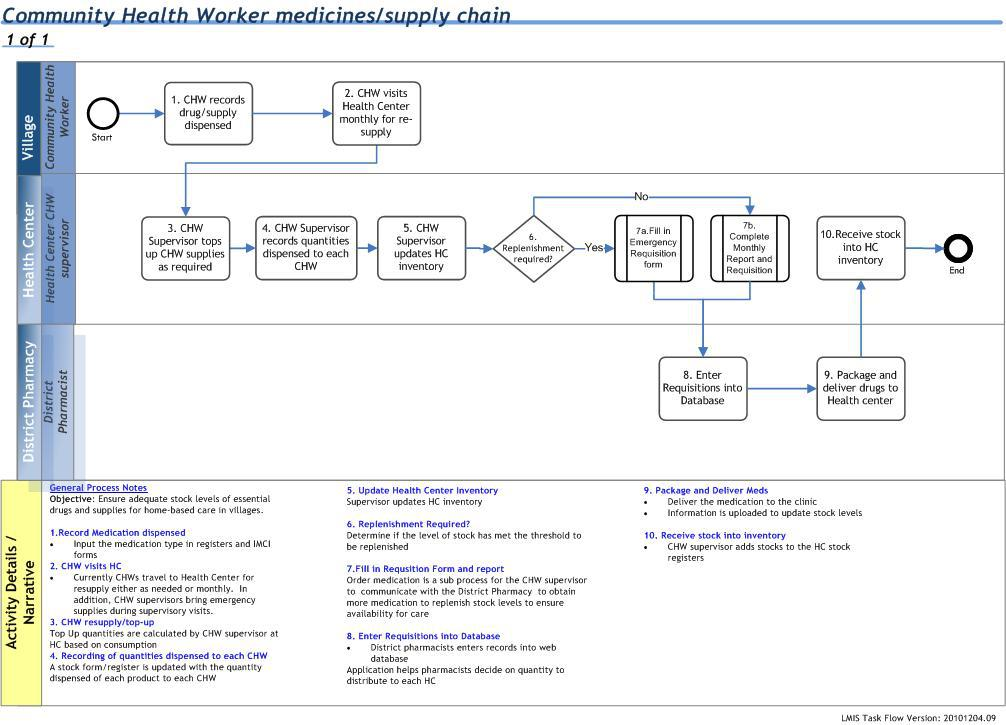
\includegraphics[width=\columnwidth]{sources/chwSupplyChain.jpg}
\label{fig:chwsc}
\caption{Community Health Worker Supply Chain}
\end{figure}

\section{Problem to be solved}
At this time the HMIS does not have access to data at a village level on essential drugs.
The HMIS would like to have access to this data and be able to provide the following services.

\begin{description}
\item[\#1] Send SMS and email notifications based on rules.
\item[\#2] Send SMS and email reminder if a report is more than 4 days delayed.
\item[\#3] If user data does not map correctly user feedback should be provided.
\item[\#4] A functional SMS based reporting system.
\end{description}


\chapter{Proposed Solution}

\section{Use Cases}

\subsection{Notifications}

Based on collected data and the prediction algorithm ,'Cell CHW Supervisor', 'HC CHW Supervisor' and 'District Pharmacist' will be notified of how much of the essential drugs is needed at the level below their own in the administrative hierarchy for a given period. 

\begin{table}[h]
	\centering
	\begin{tabular}{|l|l|}
		\hline
		\multicolumn{2}{|c|}{\textbf{Send SMS and Email Notifications}}\\
		\hline
		\textbf{Goal:} & Create orders\\
		\hline
		\textbf{Primary Actor:} & System\\
		\hline
		\multirow{3}{*}{\textbf{Secondary Actor:}}	& Cell CHW Supervisor \\
																								& HC CHW Supervisor \\ 
																								& District Pharmacist \\
		\hline
		\multirow{4}{*}{\textbf{Main Success Scenario:}}	& 1. CHW reports distributed and stock values. \\
																											& 2. System processes report. \\
																											& 3. System calculates essential drugs needed for each level. \\
																											& 4. System sends orders to cell, sector and district. \\
		\hline
		\textbf{Extensions:} & \\
		\hline
	\end{tabular}
	\caption{Textual Use Case: Send SMS and Email Notifications}
\end{table}
\pagebreak

\subsection{Reminders}

If a 'CHW' report is more than 5 days late the 'System' should send a reminder to the 'CHW' responsible. If the report is more than 10 days late, the 'System' will send a reminder to the 'Cell CHW Supervisor' responsible for the  same village.

\begin{table}[h]
	\centering
	\begin{tabular}{|l|l|}
		\hline
		\multicolumn{2}{|c|}{\textbf{Send SMS and Email Reminders}}\\
		\hline
		\textbf{Goal:} & Send reminder \\
		\hline
		\textbf{Primary Actor:} & System \\
		\hline
		\multirow{2}{*}{\textbf{Secondary Actor:}}	& CHW \\
																								& Cell CHW Supervisor \\
		\hline
		\multirow{5}{*}{\textbf{Main Success Scenario:}}	& 1. CHW misses report deadline. \\
																											& 2. 5 days goes by. \\
																											& 3. System sends reminder by email and SMS. \\
																											& 4. Another 5 days goes by. \\
																											& 5. System sends reminder by email and SMS. \\
																											
		\hline
		\textbf{Extensions:} & \\
		\hline
	\end{tabular}
	\caption{Textual Use Case: Send SMS and Email Reminders}
\end{table}
\pagebreak

\subsection{Feedback}

Given that a 'CHW' has reported data that does not map correctly, a message containing what went wrong and the necessary steps in order to correct the report will be sent back to the 'CHW'.

\begin{table}[h]
	\centering
	\begin{tabular}{|l|l|}
		\hline
		\multicolumn{2}{|c|}{\textbf{Send Report Feedback}} \\
		\hline
		\textbf{Goal:} & Process SMS message\\
		\hline
		\textbf{Primary Actor:} & System \\
		\hline
		\textbf{Secondary Actor:} & Community Health Worker \\
		\hline
		\multirow{6}{*}{\textbf{Main Success Scenario:}}	& 1. CHW reports data incorrectly by SMS. \\
																											& 2. System receives SMS. \\
																											& 3. SMS triggers feedback message. \\
																											& 4. CHW corrects message and re-sends report. \\
																											& 5. System processes SMS. \\
																											& 6. System updates database. \\
		\hline
		\textbf{Extensions:} & \\
		\hline
	\end{tabular}
	\caption{Textual Use Case: Send Report Feedback}
\end{table}
\pagebreak

\subsection{Reporting}

A 'CHW' will be able to report by SMS, stock and distributed values of essential drugs at a village level in the administrative hierarchy. 

\begin{table}[h]
	\centering
	\begin{tabular}{|l|l|}
		\hline
		\multicolumn{2}{|c|}{\textbf{Report Using SMS}}\\
		\hline
		\textbf{Goal:} & Update Database \\
		\hline
		\textbf{Primary Actor:} & Community Health Worker\\
		\hline
		\textbf{Secondary Actor:} & System \\
		\hline
		\multirow{5}{*}{\textbf{Main Success Scenario:}}	& 1. CHW reports stock and distributed values of essential drugs. \\
																											& 2. System receives SMS. \\
																											& 3. System processes SMS. \\
																											& 4. System updates database. \\
																											& 5. System sends confirmation SMS to CHW. \\
		\hline
		\textbf{Extensions:} & \\
		\hline
	\end{tabular}
	\caption{Textual Use Case: Report Using SMS}
\end{table}
\pagebreak

\begin{figure}
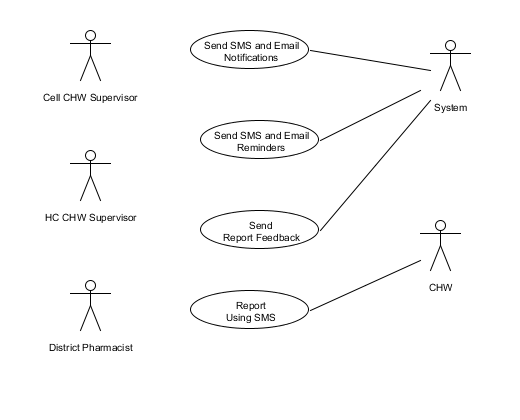
\includegraphics[width=\columnwidth]{img/hmisReq.png}
\label{fig:use_case}
\caption{Use Case Diagram}
\end{figure}

\begin{figure}
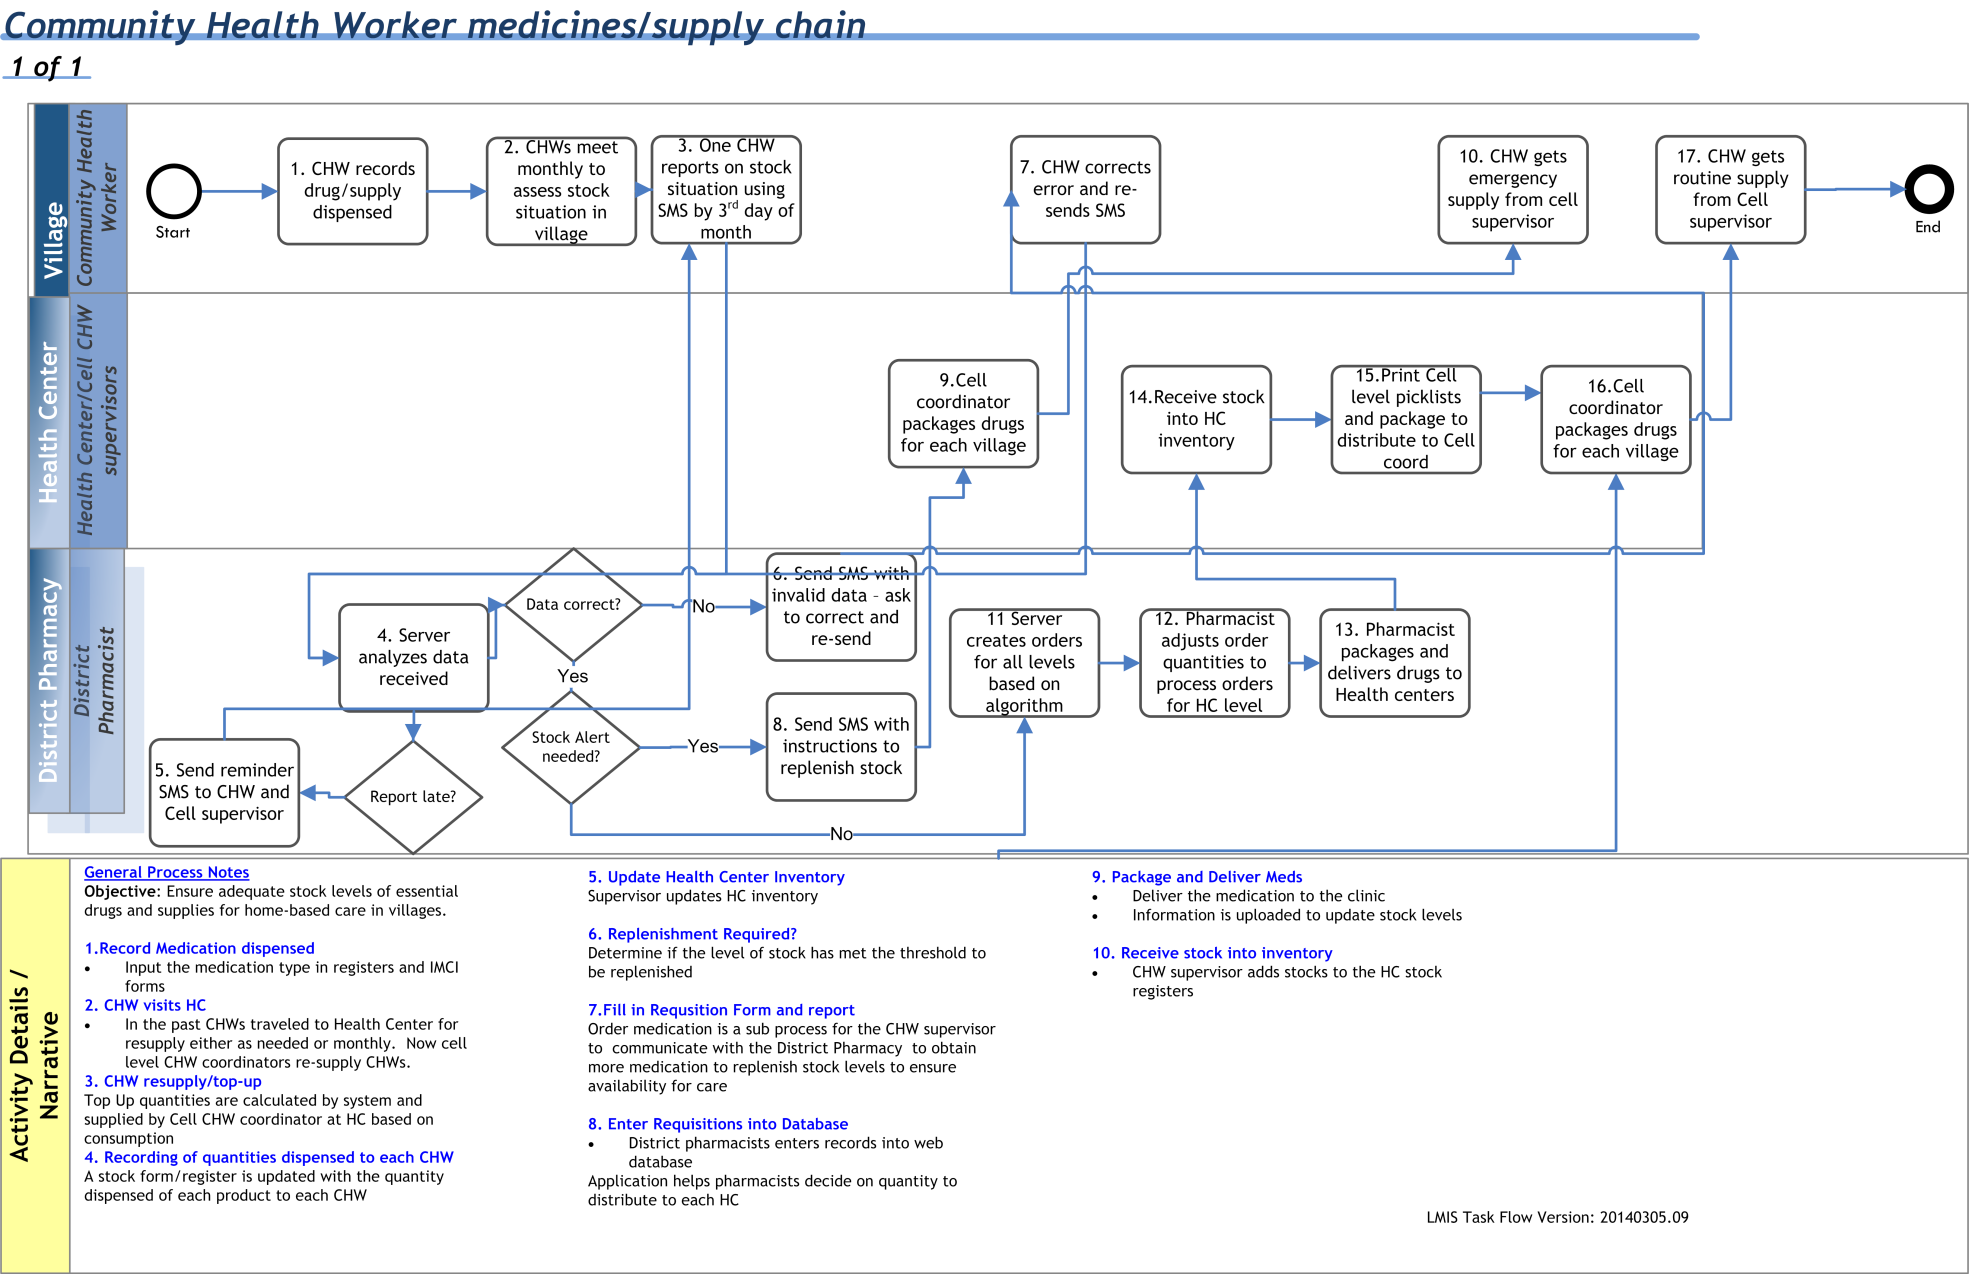
\includegraphics[width=\columnwidth]{img/supplyChain.png}
\label{fig:supplychainsolution}
\caption{Community Health Worker Supply Chain}
\end{figure}


\chapter{Test Environment}
\section{Local DHIS2 and Windows}

\begin{table}
	\centering
	\begin{tabular}{|l|l|}
		\hline
		Operating System: & Windows 7 Professional Service Pack 1 \\
		\hline
		Processor: & Intel(R) Core(TM) i7-2630QM CPU @ 2.00GHz \\
		\hline
		RAM: & 4.00GB \\
		\hline
		System type: & 64bit \\
		\hline
		Web Server: & Apache Tomcat Version 8.0.3 \\
		\hline
		Database: & PostgreSQL 9.2.4 \\
		\hline
		Software: & DHIS2 2.14 \\
		\hline
	\end{tabular}
	\caption{System Description}
\end{table}
\begin{table}
	\centering
	\begin{tabular}{|l|p{13cm}|}
		\hline
		\multicolumn{2}{|c|}{\textbf{Environment Variables}} \\
		\hline
		\multirow{3}{*}{PATH:}	& C:\textbackslash Program Files\textbackslash Java\textbackslash jdk1.7.0\_25\textbackslash bin; \\
														& C:\textbackslash Program Files\textbackslash Apache Software Foundation\textbackslash apache-maven-3.1.0\textbackslash bin; \\
														& C:\textbackslash Program Files\textbackslash PostgreSQL\textbackslash 9.2\textbackslash bin; \\
		\hline
		DHIS2\_HOME: & C:\textbackslash Program Files\textbackslash Apache Software Foundation\textbackslash apache-tomcat-8.0.3\textbackslash conf \\
		\hline
		JAVA\_HOME: & C:\textbackslash Program Files\textbackslash Java\textbackslash jdk1.7.0\_25 \\
		\hline
		JAVA\_OPTS: & -Xms512m -Xmx1024m -XX:MaxPermSize=256M \\
		\hline
		M2: 				& C:\textbackslash Program Files\textbackslash Apache Software Foundation\textbackslash apache-maven-3.1.0\textbackslash bin \\
		\hline
		M2\_HOME: 	& C:\textbackslash Program Files\textbackslash Apache Software Foundation\textbackslash apache-maven-3.1.0 \\
		\hline
		MAVEN\_OPTS	& -Xms512m -Xmx1024m -XX:MaxPermSize=256M \\
		\hline
	\end{tabular}
	\caption{Example: Environment Variables}
\end{table}

\subsection{Setting environment variables}
Windows requires some of the environments variables to be set.


\subsection{Launch DHIS2 with Tomcat}

\subsection{Organization Unit}

\subsection{Users}
\subsubsection{Create test user}
\subsubsection{Import users}
\subsubsection{Assign user to organization unit}

\subsection{Data}
\subsubsection{Create data elements}
\subsubsection{Create data set}
\subsubsection{Assign data set to organization unit}


\subsection{SMS}
\subsubsection{Create SMS command}
\subsubsection{Start SMS service}
\subsubsection{Test with integrated 'testSMS.action'}

\end{document}

\section{Local DHIS2 instance, Windows and Android App}

\section{DHIS2 instance at the national data center}
